\documentclass[aspectratio=169]{beamer}
\usepackage[utf8]{inputenc}
\usepackage[style=authoryear,backend=biber]{biblatex}
\usepackage{amsmath}
\addbibresource{main.bib}
\usetheme{Madrid}
\usecolortheme{default}
\usepackage{dutchcal}
\usepackage{enumitem}
\usepackage{graphicx}
\usepackage{algorithm}
\usepackage{algpseudocode}
\usepackage{jm}
\usepackage{multicol}


%------------------------------------------------------------
%This block of code defines the information to appear in the
%Title page
\title[Facility Location w. Drones] %optional
{Drone Delivery System in Post-Disaster Humanitarian Logistics: A
Two-Stage Stochastic Programming Approach with Uncertain Wind
Conditions}

% \subtitle{A brief introduction}

\author[Yuyang Ma] % (optional)
{Yuyang Ma}

\institute[ISE] % (optional)
{
  Department of Industrial and Systems Engineering\\
  Lehigh University
}

\date[Jun 13 2024] % (optional)
{Qualifying Exam Presentation, June 2024}

\logo{
\includegraphics[height=1cm]{LU.png}}

%End of title page configuration block
%------------------------------------------------------------
%------------------------------------------------------------
%The next block of commands puts the table of contents at the 
%beginning of each section and highlights the current section:

\AtBeginSection[]
{
  \begin{frame}
    \frametitle{Table of Contents}
    \tableofcontents[currentsection]
  \end{frame}
}
%------------------------------------------------------------
\begin{document}
\newcommand{\hltblue}[1]{\textcolor{blue}{#1}}
\newcommand{\hltred}[1]{\textcolor{red}{#1}}

%The next statement creates the title page.
\frame{\titlepage}
%---------------------------------------------------------
%This block of code is for the table of contents after
%the title page
\begin{frame}
\frametitle{Contents}
\tableofcontents
\end{frame}
%---------------------------------------------------------
% Slide 1: Introduction
\section{Introduction}
\begin{frame}
    \frametitle{Introduction}
    \begin{itemize}
      \item \textbf{UAVs for Humanitarian Logistics:} Exploration by leading companies like DHL \footcite{dhl2018drone} and Zipline \footcite{Zipline2020} for medicine deliveries, highlighting the growing interest in drone technology.
      \item \textbf{Technological Advances:} Significant improvements in drone materials, sensing and coordination algorithms, battery life, and regulatory frameworks are propelling UAV adoption.
      \item \textbf{Facility Location Challenge:} The central issue of limited range and payload capacity of drones necessitates strategic planning for the placement of depots or launching sites.
      \item \textbf{Solution Model:} Introduction of a two-stage stochastic programming model focusing on selecting optimal locations for drone launching facilities, and size of drones' fleet to meet spatially distributed affected people's demands efficiently. The detailed formulation will be shown in next section.
    \end{itemize}
\end{frame}

% Slide 2: Benefits and Challenges of Drone Deliveries
\begin{frame}{Benefits and Challenges of Drone Deliveries}
  \begin{columns}
    \column{0.45\textwidth}
    \textbf{Benefits of Using Drones:}
    \begin{itemize}
      \item Improved Accessibility
      \item Efficiency and Safety
      \item Real World Applications
    \end{itemize}
    
    \column{0.45\textwidth}
    \textbf{Challenges of Drone Deliveries:}
    \begin{itemize}
      \item Limited Range and Payload
      \item Weather Susceptibility
      \item Computational Complexity
    \end{itemize}
  \end{columns}
\end{frame}

% Slide 3: Literature Review
\begin{frame}
\frametitle{Literature Review}
    \begin{enumerate}[label=\arabic*.]
        \item \textbf{Routing Problem:} 
        \begin{itemize}[label=$\star$]
          \item Murray and Chu (2015) \cite{murray2015flying} proposed two kinds of routing problems:
          \begin{itemize}[label=$\diamond$]
            \item \text{Flying Sidekick Traveling Salesman Problem (FSTSP)}
            \item \text{Parallel Drone-Scheduling Traveling Salesman Problem}
          \end{itemize}
          \item Murray and Raj (2020)\cite{murray2020multiple} extended the FSTSP with multiple drones during the delivery.
        \end{itemize}
        \item \textbf{Facility Location Problem:}
        \begin{itemize}[label=$\diamond$] 
          \item Chauhan et al. (2019) \cite{chauhan2019maximum} proposed a maximal covering facility location model with drones (MCFLPD).
        \end{itemize}
        \item \textbf{Delivery with Uncertainties:}
        \begin{itemize}[label=$\diamond$]
          \item Zhu et al. (2022) \cite{zhu2022two} incorporated demand uncertainty with a two-stage robust optimization model.
          \item Cheng et al. (2024) \cite{cheng2024robust} considered uncertain wind conditions in a drone delivery system.
        \end{itemize}
    \end{enumerate}
\end{frame}

% Slide 4: Review on the original paper
\begin{frame}{Review on Dukkanci et al. (2023)\footcite{dukkanci2023drones}}
  \begin{itemize}
    \item \textbf{Topic:} Using drones to distribute relief supplies in post-disaster scenarios
    \item \textbf{Objective:} Selecting optimal locations for drone launching facilities to minimize unmet demands of affected people
    \item \textbf{Methodology:} Two-stage mixed-integer stochastic programming model
    \item \textbf{Contributions:} 
      \begin{enumerate}[label=\arabic*.]
        \item Featured an endogenous drone range and time-bound constraints into the model
        \item Considered the uncertain road network and demand induced by disasters
        \item Proposed a scenario decomposition algorithm (SDA) to solve the problem
        \item Conducted a real-world case study to validate the model
      \end{enumerate}
    \item \textbf{Room for Improvements:} Fairness issues in distribution, weather uncertainties, unrealistic assumptions, etc.
  \end{itemize}
\end{frame}

% Slide 6: Problem Statement and Model Formulation
\section{Problem Statement and Model Formulation}
\subsection{Problem Statement}
\begin{frame}
    \frametitle{Problem Statement}
    In this study, we extend the model proposed by Dukkanci et al. (2023) \footcites{dukkanci2023drones}. The objective is to minimize the total cost of the drone delivery system while ensuring that the unmet demand of affected people is minimized. The detailed statement is listed as follows:
    \begin{enumerate}[label=\arabic*.]
        \item Given a set of locations for gathering points $I$, potential launch points $L$ and potential depots $D$. Sets of available fully-charged drones are: $K_{SD}$ for small drones and $K_{LD}$ for large drones. 
        \item Decide to open at most $p$ launch points and $e$ depots. Assign each open launch point to one open depot.
        \item Disaster (earthquake in our study) happens. Damage percentage of road networks, demands at gathering points, and wind conditions are observed.
        \item Determine the size of drone fleets. Assign drones to open facilities (launch points or depots) for serving the gathering points. All deliveries must be finished within $T$ hours. 
    \end{enumerate}
\end{frame}

% Slide 5: A sample graph
\begin{frame}{A Sample Graph for Two-Echelon Delivery System}
    In Dukkanci et al. (2023), they proposed a two-echelon delivery system, where trucks and drones cooperated to distribute the relief items after the disaster. A sample graph of proposed delivery system is illustrated as follows:
    \begin{figure}[h]
        \centering
        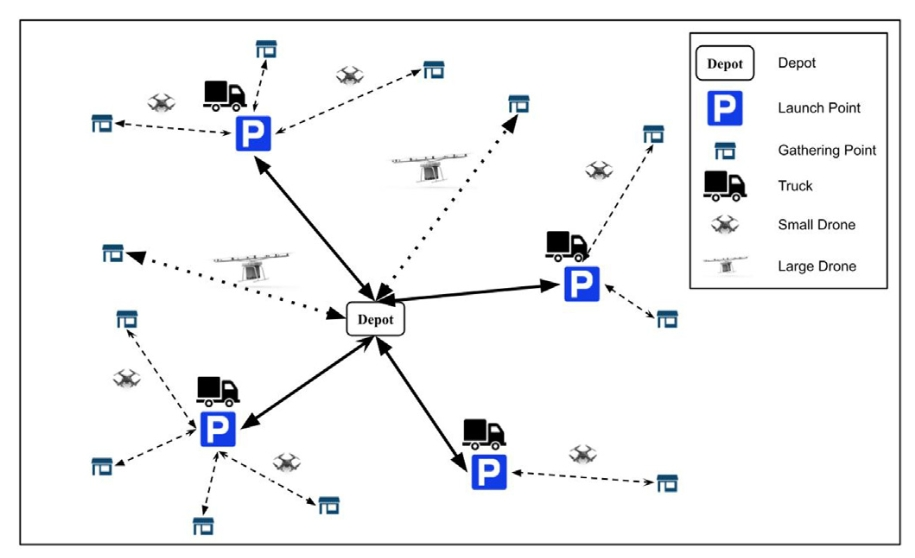
\includegraphics[width=0.4\textwidth]{Drone_delivery_system.png}
        \caption{Two-Echelon Delivery System \footcite{dukkanci2023drones}}
        \label{fig:delivery_system}
    \end{figure}
\end{frame}

\subsection{Mathematical Notation and Formulation}
% Slide 7: Mathematical Notation
\begin{frame}{Mathematical Notations I}
\scriptsize
\centering
    \begin{tabular}{ll}
        \hline
        \textbf{Parameters} & \textbf{Description} \\
        \hline
        $e$ & Maximal number for open depots \\
        $p$ & Maximal number for open launch points \\
        $Q_T$ & Capacity of trucks \\
        $Q_{SD}$ & Capacity of small drones \\
        $Q_{LD}$ & Capacity of large drones \\
        $c_{SD}$ & Cost of using small drones \\
        $c_{LD}$ & Cost of using large drones \\
        $v_T$ & Speed of trucks \\
        $v_{SD}$ & Speed of small drones \\
        $v_{LD}$ & Speed of large drones \\
        $v^w$ & Speed of wind \\
        $\alpha^w$ & Direction of wind \\
        $T$ & Length of time period \\
        $\tau$ & Preparation time for small drones \\
        $w_{dl}$ & Ground distance between depot $d$ and launch point $l$ after the earthquake \\
        $q_i$ & Demand at gathering point $i$ \\
        $\pi$ & Penalty per unit of unmet demand \\
        \hline
    \end{tabular}
\end{frame}

% Slide 8: Mathematical Notation II
\begin{frame}{Mathematical Notation II}
    \begin{itemize}
        \item \textbf{First-Stage Decision Variables}
        \begin{itemize}
            \item $u_d$: 1, if a depot is open at location $d \in D$, 0 otherwise
            \item $v_l$: 1, if a launch point is open at location $l \in L$, 0 otherwise
            \item $w_{dl}$: 1, if launch point $l$ is assigned to depot $d$, 0 otherwise
        \end{itemize}
        \item \textbf{Second-Stage Decision Variables}
        \begin{itemize}
            \item $g_k$: 1, if a drone $k \in \{K_{SD} \cup K_{LD}\}$ is used, 0 otherwise
            \item $x_{ilk}$: 1, if a small drone $k \in K_{SD}$ is assigned to serve point $i \in I$ from location $l \in \{L \cup D\}$, 0 otherwise
            \item $y_{idk}$: 1, if a large drone $k \in K_{LD}$ is assigned to serve point $i \in I$ from depot $d \in D$, 0 otherwise
            \item $o_i$: Unmet demand for gathering point $i \in I$
        \end{itemize}
    \end{itemize}
\end{frame}

% Slide 9: First-Stage Problem
\begin{frame}
\frametitle{Two-Stage Stochastic Programming I}
\begin{alertblock}{First-Stage Problem}
\small
Objective: minimize the expectation the second stage's cost $Q$.
\scriptsize
\vspace{-3pt}
    \begin{subequations} \label{formulation:1stStage}
        \begin{align}
            \min \quad & \Embb_{\Pmbb} \left[ Q(u,v,w,\xi) \right] && \label{objective:1stStageObj} \\
            \subjectto \quad & \sum_{d \in D} u_d \leq e,     && \label{constraint:Num_Depot} \\
                             & \sum_{l \in L} v_l \leq p,     && \label{constraint:Num_Launch} \\
                             & \sum_{d \in D} w_{ld} = v_l,  && \forall l \in L \label{constraint:LaunchPointtoOneDepot} \\
                             & w_{ld}, u_d, v_l \in \{0,1\}. && \forall d \in D, l \in L \label{constraint:wBinary}
        \end{align}
    \end{subequations}
\end{alertblock}
\begin{block}{Notation}
    The uncertainties in the second-stage are indicated as the parameter $\xi \in \Xi$, where $\xi = \left( \omega, q , v^{wind} , \alpha^{wind} \right)$, and $\Pmbb$ is a known probability distribution of $\xi$.   
\end{block}
\end{frame}

% Slide 10: Second-Stage Problem
\begin{frame}
    \frametitle{Two-Stage Stochastic Programming II}
    \begin{alertblock}{Second-Stage Problem}
    \small
    Objective: total cost of using drones and the penalty of unmet demand.
    \tiny
    \vspace{-5pt}
    \begin{subequations} \label{formulation:2ndStage}
        \begin{align}
            Q[u,v,w,\xi] :=  \quad \min \quad & \sum_{i \in I} \pi o_i + \sum_{k \in K_{SD}} c_{SD} g_k + \sum_{k \in K_{LD}} c_{LD} g_k & & \label{objective:2ndStageObj} \\
                         \subjectto \quad & \text{Constraints for open depots, launch points, and using drones} \\
                                          & \sum_{k \in K_{SD}} \sum_{i \in I} q_i x_{ilk} \leq Q_T v_l && \forall l \in L \label{constraint:TrucksCapacity} \\
                                          & q_i - \sum_{k \in K_{SD}}\sum_{l \in \{L \cup D\}} Q_{SD} x_{ilk} - \sum_{k \in K_{LD}}\sum_{d \in D} Q_{LD} y_{idk} \leq o_i && \forall i \in I \label{constraint:UnmetDemand} \\
                                          & \sum_{d \in D} \frac{\omega_{ld}}{v_T} w_{ld} + \sum_{i \in I} \left( \frac{2d_{li}}{v_{li}} + \tau \right) x_{ilk} \leq T && \forall l \in L, k \in K_{SD} \label{constraint:LPTimeLimitSD} \\
                                          & \sum_{i \in I} \left( \frac{2d_{li}}{v_{li}} + \tau \right) x_{ilk} \leq T && \forall l \in D, k \in K_{SD} \label{constraint:DepotTimeLimitSD} \\
                                          & \frac{2d_{ji}}{v_{ji}} y_{ijk} \leq T && \forall j \in D, i \in I, k \in K_{LD} \label{constraint:DepotTimeLimitLD} \\
                                          & g_k \geq g_{k+1} && \forall k, k+1 \in K_{SD} \label{constraint:SD_Remove_Symmetry} \\
                                          & g_k \geq g_{k+1} && \forall k, k+1 \in K_{LD} \label{constraint:LD_Remove_Symmetry} 
        \end{align}
    \end{subequations}
    \end{alertblock}
\end{frame}

% Slide 11: Speed Calculation
\begin{frame}{Maximal Average Speed Calculation for Drones}
In this study, we use the following formula proposed by Dukkanci et al.\footcites{dukkanci2021energyandcost} to calculate the maximal average speed for drones to deliver from facility $l$ to gathering point $i$:
\begin{equation}
    R(v) \triangleq \frac{\Theta}{\frac{\mu_1}{v} + \mu_2 v + \frac{\mu_3}{v^2} + \mu_4 v^2}, \label{eq:range_speed_formula}
\end{equation}
where parameters $\mu_1$, $\mu_2$, $\mu_3$, $\mu_4$, and $\Theta$ are constants that depend on the drone model, and the detailed calculation is listed in the supplementary materials. \\
\vspace{1em}
In practice, we set $R(v) = 2 \times d_{il}$, where $d_{il}$ is the air line distance between facility $l$ and gathering point $i$, which will not be affected by the disaster.
\end{frame}


% Slide 12: Uncertain Wind Conditions
\subsection{Uncertain Wind Conditions}
\begin{frame}\frametitle{Affects of Wind on Delivery Process}
As proposed in Cheng et al. (2024)\footcite{cheng2024robust}, the affect of wind on the delivery process can be illustrated as follows:
\begin{figure}[h]
    \centering
    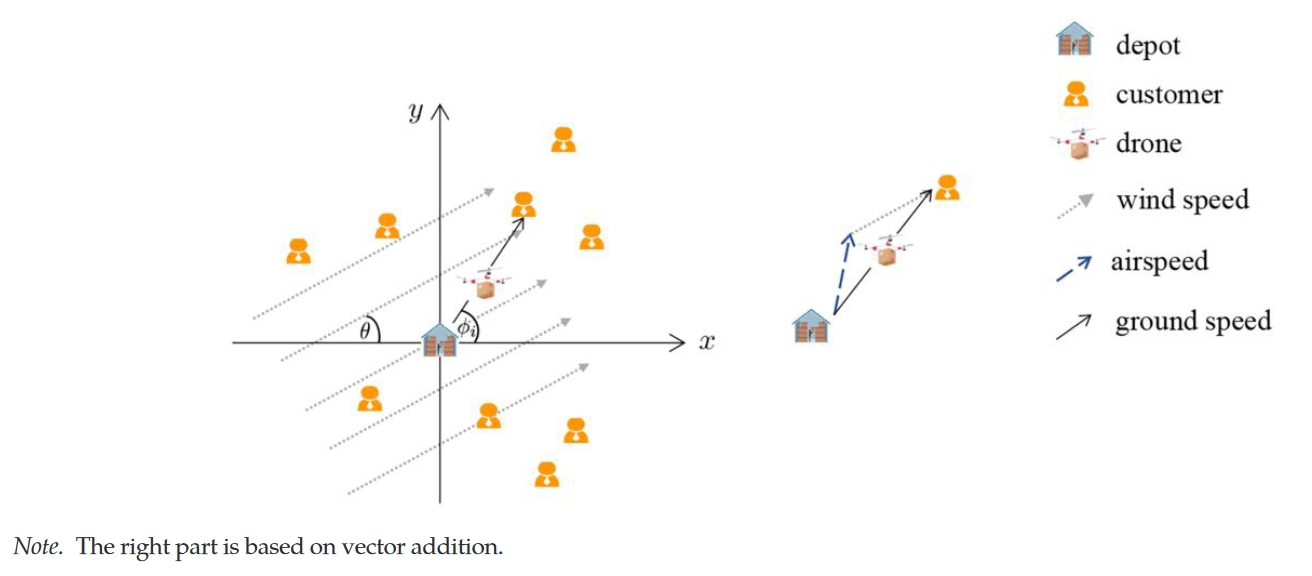
\includegraphics[width=0.5\textwidth]{figure_windspeed.png}
    \caption{Affects of Wind on Delivery Process}
    \label{fig:wind_affect}
\end{figure}
\vspace{-10pt}
For a drone $k$ is assigned to serve point $i$ from facility $l$, if maximal average speed calculate by equation \eqref{eq:range_speed_formula} $v^k_{max} \leq v^{wind}$, the drone cannot be assigned to this delivery task.
\end{frame}

\section{Solution Approaches}

\subsection{Sample Average Approximation}
% Slide 13: Sample Average Approximation
\begin{frame}
\frametitle{Sample Average Approximation}
In this study, we use the sample average approximation (SAA) method to formulate the proposed two-stage stochastic programming problem into a deterministic optimization problem.
\begin{alertblock}{Sample Average Approximation}
\vspace{-20pt}
\scriptsize
    \begin{subequations} \label{formulation:SAA}
        \begin{align}
            \min \quad & \frac{1}{|S|} \sum_{s \in S} \left(\sum_{i \in I} \pi o_{s,i} + \sum_{k \in K_{SD}} c_{SD} g_{s,k} + \sum_{k \in K_{LD}} c_{LD} g_{s,k} \right) && \label{objective:SAAObj} \\
            \subjectto \quad & \text{Constraints (\ref{constraint:Num_Depot}) - (\ref{constraint:wBinary})} && \label{constraint:1stStage_SAA}\\
                            & \vdots \\
                            & \sum_{d \in D} \frac{\omega_{sld}}{v_T} w_{ld} + \sum_{i \in I} \left( \frac{2d_{li}}{v_{sli}} + \tau \right) x_{silk} \leq T && s \in S , \forall l \in L, k \in K_{SD} \label{constraint:LPTimeLimitSD_SAA} \\
                            & \vdots \\
                            & g_{s,k} \geq g_{s,k+1} && \forall s \in S , k, k+1 \in K_{SD} \label{constraint:SD_Remove_Symmetry_SAA} \\
                            & g_{s,k} \geq g_{s,k+1} && \forall s \in S , k, k+1 \in K_{LD} \label{constraint:LD_Remove_Symmetry_SAA}
        \end{align}
    \end{subequations}    
\end{alertblock}
\end{frame}

% Slide 14: Scenario Decomposition Algorithm
\subsection{Scenario Decomposition Algorithm (SDA)}
\begin{frame}{Intuition of Scenario Decomposition Algorithm}
\small
In stochastic programming, the nonanticipativity constraint requires that the first-stage decision must be independent of the realization of the random variable.
\scriptsize
\begin{itemize}
    \item \textbf{Phase 1: Relaxation of Nonanticipativity}
    \begin{itemize}[label=$\diamond$] 
        \item During the first phase, the nonanticipativity of the first-stage decision variables is relaxed.
        \item This relaxation enables the decomposition of the problem into individual scenarios.
        \item Each scenario is treated as a deterministic problem.
        \item Solving these yields a lower bound for the main problem based on the optimal values from the single-scenario problems.
    \end{itemize}
    \item \textbf{Phase 2: Fixing First-Stage Variables}
    \begin{itemize}[label=$\diamond$] 
        \item In the second phase, the algorithm fixes the first-stage decision variables using the solutions obtained in the first phase.
        \item Solves for an upper bound for each scenario.
        \item The upper bound for the main problem is derived by considering the expected value of the single-scenario solutions.
    \end{itemize}
\end{itemize}
\small
Repeat the two phases until the upper bound converges to the lower bound, where the relaxed nonanticipativity constraints are satisfied.
\end{frame}

% Slide 15: Scenario Decomposition Algorithm
\begin{frame}{Pseudocode of Scenario Decomposition Algorithm}
\vspace{-10pt}
    \begin{algorithm}[H]
        \caption{Scenario decomposition algorithm} \label{alg:SDA}
        \begin{algorithmic}[1]
        \tiny
        \State \textbf{initialize:} $UB \gets +\infty, LB \gets -\infty, R \gets \emptyset, x^* \gets 0, y^* \gets 0, w^* \gets 0$
        \While {$UB > LB$ and $\{0,1\}^{(D+L+DL)} \setminus R \neq \emptyset$}
            \For {$s = 1$ to $S$}
                \State solve the \textit{relaxation} of the second stage formulation including constraints to exclude existing solutions
                \State let $(\bar{x}_s, \bar{y}_s, \bar{w}_s)$ be the optimal solution and $lb_s$ be the optimal objective value
            \EndFor
            \State $LB \gets \sum_{s=1}^S p_s lb_s$, $\hat{R} \gets \bigcup_{s=1}^S \{\bar{x}_s, \bar{y}_s, \bar{w}_s\}$, $R \gets R \cup \hat{R}$
            \For {$\{x, y, w\} \in \hat{R}$}
                \State $u \gets 0$
                \For {$s = 1$ to $S$}
                    \State solve the problem formulation given $x, y,$ and $w$ variables; let $f_s(x, y, w)$ be the optimal objective value
                    \If {Problem is infeasible}
                        \State set $f_s(x, y, w) \gets \infty$ and $u \gets \infty$
                    \Else
                        \State set $u \gets u + p_s f_s(x, y, w)$
                    \EndIf
                \EndFor
                \If {$UB > u$}
                    \State $UB \gets u, x^* \gets x, y^* \gets y$ and $w^* \gets w$
                \EndIf
            \EndFor
        \EndWhile
        \end{algorithmic}
    \end{algorithm}
\end{frame}

\subsection{Cluster-Based Heuristic Algorithm}
% Slide 16: Intuition Cluster-Based Heuristic Algorithm
\begin{frame}{Intuition of Cluster-Based Heuristic Algorithm}
Although the objective function depends on second-stage decision variables, the decisions made in the first-stage, locations for open drone facilities, implicitly affect the objective function for the following reasons:
\begin{enumerate}[label=\arabic*.]
    \item Range limit of drones and time window restrictions affect coverage.
    \item Location of drone facilities is critical.
    \item First-stage decision variables implicitly affect the objective function.
    \item Despite disruptions, aerial distances remain unchanged.
\end{enumerate}
\vspace{1em}
Moreover, we assume that there are more open launch points than depots. Therefore, we prioritize \textcolor{blue}{distance between launch points and gathering points} over \textcolor{red}{distance between depots and gathering points}.
\end{frame}

% Slide 17 ~ 18: Cluster-Based Heuristic Algorithm
\begin{frame}{Cluster-Based Heuristic Algorithm (Steps 1-4)}
\Large
Full steps of the cluster-based heuristic algorithm are listed as follows:
\normalsize
\vspace{1em}
    \setlist[enumerate,1]{label=Step \arabic*., leftmargin=*, labelwidth=4em, topsep=0em, itemsep=1em, parsep=1em}
    \begin{enumerate}[itemsep=0em]
        \item \textcolor{blue}{Using $k$-means algorithm to cluster the gathering points into $p$ clusters}, where $p$ is the maximal number of open launch points.
        \item For each launch point, calculate the total distance between the launch point and all gathering points in a cluster and \textcolor{blue}{assign the launch points to the cluster with the smallest total distance.}
        \item Among all launch points in the same cluster, \textcolor{blue}{select the one with the smallest total distance to the gathering points as the open launch point.}
        \item \textcolor{blue}{Using $k$-means algorithm to cluster all open launch points into $e$ clusters}, where $e$ is the maximal number of open depots.
    \end{enumerate}
\end{frame}

\begin{frame}{Cluster-Based Heuristic Algorithm (Steps 5-8)}
    \setlist[enumerate,1]{label=Step \arabic*., leftmargin=*, labelwidth=4em, topsep=0em, itemsep=1em, parsep=1em}
    \begin{enumerate}[resume, start=5,itemsep=0em]
        \item For each depot, calculate the \hltblue{total distance between the depot and all open launch points in a cluster} and the \hltblue{total distance to the gathering points assigned to those launch points}. Assign the depots to the cluster with the \hltred{smallest total distance}.
        \item Among all depots in the same cluster, \hltblue{select the one with the smallest total distance to the open launch points as the open depot.}
        \item The value of the first-stage decision variables \hltblue{$u_d$ and $v_l$ are determined by the open depots and launch points}, and the \hltblue{assignment of launch points to depots}.
        \item \hltblue{Fix the value of the first-stage decision variables} and solve the second-stage problem in \hltred{each scenario}. Average the objective value of all scenarios as the optimal solution.
    \end{enumerate}
\end{frame}

\section{Computational Experiments}
\begin{frame}{Road Distance after Earthquake I}
In Erbeyoglu and Bilge (2020) \footcite{erbeyouglu2020earthquake}, they evaluated four intensity predictive models that can be applied to estimate the damage for all potential earthquakes:
\begin{subequations}
    \begin{align}
    I_s &= 7.023 + 0.703 M_s - 2.826  \log_{10}(R_{epi}), \label{eq:MSK_1} \\
    I_s &= 5.002 + 0.75 M_s - 0.0094  R_{epi} - 1.454 \log_{10}(R_{epi}) \label{eq:MSK_2}, \\
    I_s &= 7.494 + 0.744 M_s - 3.377 \log_{10} \sqrt[3]{R_{epi}^3 + h^3} + 0.017 h \label{eq:MSK_3}, \\
    I_s &= 2.281 + 0.874 M_s - 0.618 \log_{10} \sqrt{1+\frac{R_{epi}^2}{h^2}} - 0.016 \left(\sqrt{h^2 + R_{epi}^2} - h\right) \label{eq:MSK_4},
    \end{align}
\end{subequations}
where $I_s$ indicates \hltred{intensity of the earthquake}, $R_{epi}$ refers to \hltred{distance between the epicenter and the facility location}, $M_s$ represents the \hltred{surface-wave magnitude} and $h$ is \hltred{hypocentral depth of the earthquake.} 
\end{frame}

\begin{frame}{Road Distance after Earthquake II}
The average of the intensity values from the formulas \eqref{eq:MSK_1} - \eqref{eq:MSK_4} is used as the final intensity value for a certain facility and we can estimate how severe the damage is at each facility location using figure \ref{fig:MSK_scale}:
\begin{figure}
    \centering
    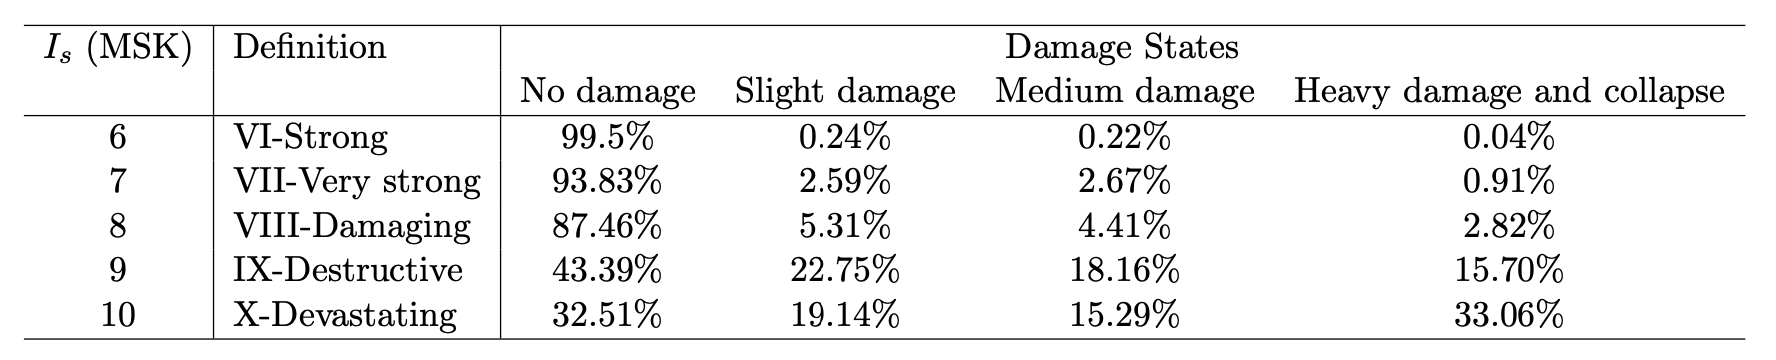
\includegraphics[width=0.8\textwidth]{eq_tab.png}
    \vspace{-10pt}
    \caption{MSK Scale for Earthquake Intensity}
    \label{fig:MSK_scale}
\end{figure}
\vspace{-5pt}
We calculate the damage percentages of each depot/launch points and consider their \hltred{average} and \hltblue{increase the road distance by the average}. 
\end{frame}

\begin{frame}{Data Generating}
    \begin{itemize}
    \item \textbf{Data Generating:}
        \begin{itemize}[label=$\star$]
            \scriptsize
            \item Due to the unavailability of detailed realistic data, we generate the dataset using Python's random function.
            \item The dataset is based on a $300 \times 300$ grid, with each unit distance representing 1 km.
            \item Locations of gathering points, launch points, and depots are predetermined.
        \end{itemize}
    
    \item \textbf{Generated Locations}
        \begin{itemize}[label=$\star$]
            \scriptsize
            \item 25 candidate locations for launch points.
            \item 10 candidate locations for depots.
            \item 40 gathering points (same as in \cite{dukkanci2023drones}).
            \item Non-overlapping and fixed locations across different scenarios.
        \end{itemize}
    
    \item \textbf{Uncertain Parameters}
        \begin{itemize}[label=$\star$]
            \scriptsize
            \item 12 different scenarios, as used in \cite{dukkanci2023drones}.
            \item \textbf{Wind Condition:}
            \begin{itemize}[label=$\diamond$]
                \item Speed: $U(0,20)$ km/hr.
                \item Direction: $U(0,2\pi)$.
            \end{itemize}
            \item \textbf{Demand at Gathering Points:}
            \begin{itemize}[label=$\diamond$]
                \item Demand: $U(0.02,20)$ kg.
                \item Based on data from \cite{dukkanci2023drones}.
            \end{itemize}
            \item Earthquake information will be detailed in the next section.
        \end{itemize}
    \end{itemize}
\end{frame}

\begin{frame}\frametitle{Performance Evaluation for SDA and Heuristic Algorithm}
In this study, we conducted numerical experiments to evaluate the performance of the SDA and heuristic algorithm. We did 2 series of test, each with 12 scenarios. The detailed settings are listed as follows:
    \begin{itemize}[label=$\star$]
        \item maximal open launch points $e \in \{ 4, 5, 6\}$, maximal number of open depots $p \in \{1,2\}$,
        \item combination of number of available drones are of 3 bundles: $(K_{SD},K_{LD}) \in \{(10,1),(15,2),(20,3)\}$.
    \end{itemize}
\vspace{1em}
We solved the SAA formulation with 3 different methods: (1) Gurobi with default settings, (2) scenario decomposition method, and (3) heuristic algorithm. The results are shown in the following slides.
\end{frame}

\begin{frame}{Performance Evaluation Results}
\begin{figure}
    \centering
    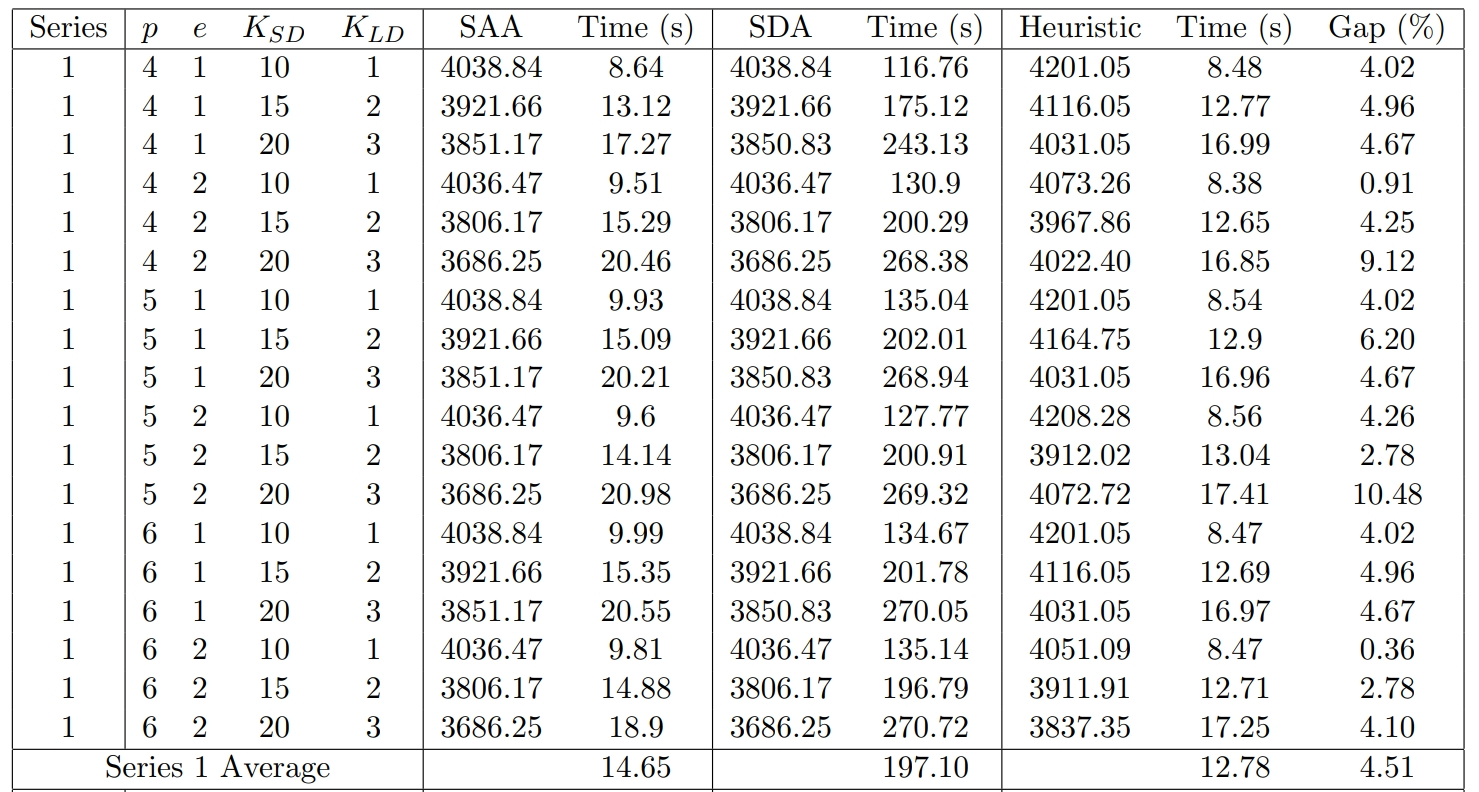
\includegraphics[width=0.7\textwidth]{fig_performance_evaluation.png}
    \caption{Part of Performance Evaluation Results}
    \label{fig:pe_result}
\end{figure}
    
\end{frame}

\begin{frame}{Large Scenario Test}
From the previous slide, it states that compared to directly using Gurobi with default settings and heuristic algorithm, the SDA takes much longer time to solve the problem. This result indicates the following facts:
\begin{itemize}
    \item[1.] the structure of the SAA formulation is not complicated;
    \item[2.] SDA performs bad in large-scale scenarios.  
\end{itemize}
To further verify the conclusion, we conducted a large scenario test. For 3 independent series of test, we increase the number of scenarios considered from 20 to 100. The results are shown in the following:
\begin{figure}
    \centering
    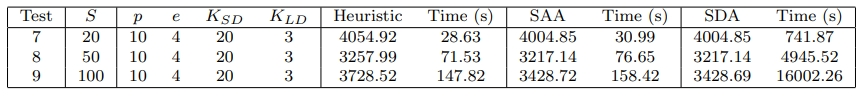
\includegraphics[width=0.7\textwidth]{fig_largeStest.png}
    \caption{Large Scenario Test Results}
    \label{fig:large_scenario}
\end{figure}
\end{frame}


\begin{frame}\frametitle{Value of Considering Weather Uncertainty}
\begin{figure}
    \centering
    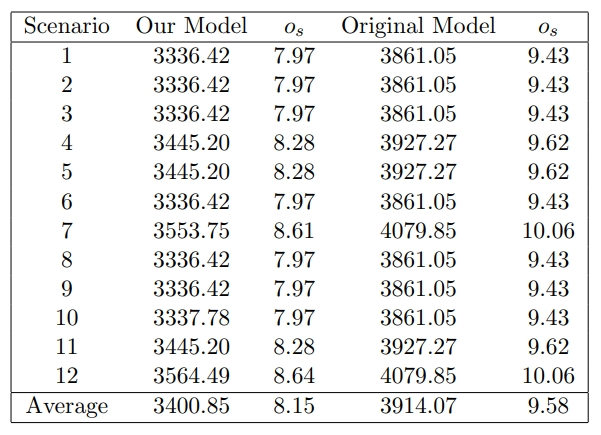
\includegraphics[width=0.35\textwidth]{fig_value_wind_uncertainty.png}
    \caption{\small Test Results Comparison: Original Model vs. Model w. Weather Uncertainty}
    \label{fig:weather_uncertainty}
\end{figure}
where $o_s$ refers to the average unmet demand for each scenario $s$. \\
\textbf{Conclusion:} the results show that considering weather uncertainty in the model leads to lower objective value and lower average unmet demand.

\end{frame}

\begin{frame}\frametitle{Impact of Fairness}
In this study, we further consider the fairness issue in the problem. To integrate the fairness into the model, we introduce 2 types of equity terms:
\begin{itemize}
    \item \textbf{Equity Constraint:} \\    
    \begin{equation}
        \scriptsize
        \sum_{k \in K_{SD}} \sum_{l \in \{L \cup D\}} x_{silk} +  \sum_{k \in K_{LD}} \sum_{d \in D} y_{sidk}\geq 1, \quad \forall i \in I, s \in S,
        \label{eq:fairness_constraint}
    \end{equation}
    The constraint ensures that each gathering point is served by at least one drone.
    \item \textbf{Penalty Term of Unfairness in Objective Function:} \\
    \begin{equation}
    \scriptsize
        \min \quad \frac{1}{|S|} \sum_{s \in S} \left(\sum_{i \in I} \pi o_{s,i} + \sum_{k \in K_{SD}} c_{SD} g_{s,k} + \sum_{k \in K_{LD}} c_{LD} g_{s,k} + \mu \left( \max_{i \in I} o_{s,i} - \min_{i \in I} o_{s,i} \right) \right),
        \label{eq:fairness_objective}
    \end{equation}
    The extra term penalizes the maximal difference in unmet demand among gathering points for each scenario.
\end{itemize}
\end{frame}

\begin{frame}{Fairness Test Results}
In this test, we set the value of parameters as follows:
\begin{enumerate}[label=\arabic*.]
    \item maximal open launch points $e = 20$, maximal number of open depots $p = 5$, $|K_{SD}| = 30$, $|K_{LD}| = 5$, Time Frame $T=2.5$ hrs;
    \item maximal solution time for Gurobi is 3000 seconds;
\end{enumerate}
\begin{figure}
    \centering
    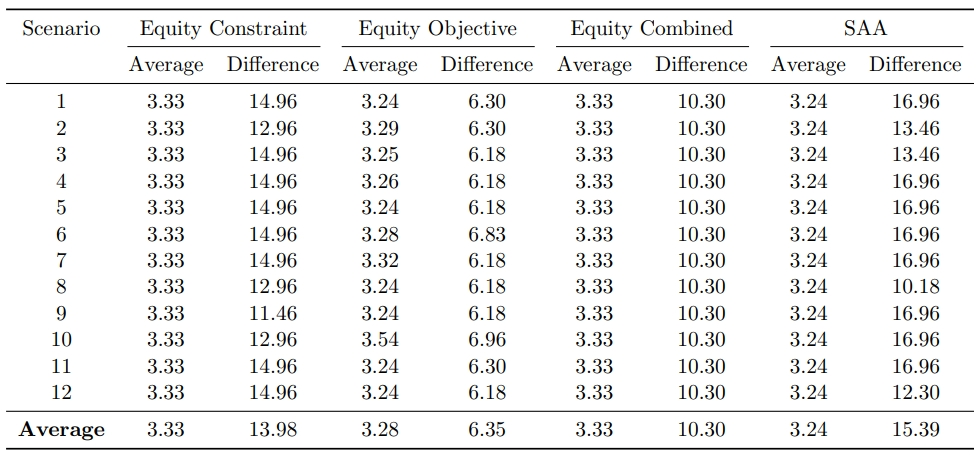
\includegraphics[width=0.6\textwidth]{fig_fairness_test.png}
    \caption{Fairness Test Results}
    \label{fig:fairness_test}
\end{figure}
\end{frame}

\begin{frame}{Discussion on Fairness Test Results}
\begin{itemize}[label=$\cdot$]
    \item The results show that the fairness constraint and penalty term significantly reduce the maximal difference in unmet demand among gathering points.
    \item However, both methods have their own advantages and disadvantages:
    \item \textbf{Fairness Constraint:} \\
    \begin{itemize}
        \item \textbf{Advantages:} Guarantees that each gathering point is served by at least one drone.
        \item \textbf{Disadvantages:} Break the nice structure, complete recourse, of the stochastic programming model.
    \end{itemize}
    \item \textbf{Penalty Term of Unfairness in Objective Function:} 
    \begin{itemize}
        \item \textbf{Advantages:} Keep the complete recourse property of the model; dramatically reduce the maximal difference in unmet demand.
        \item \textbf{Disadvantages:} Increase the complexity of the model by introducing two auxiliary decision variables, leading to a longer computation time, e.g. both model with modified objective function failed to solve within 3000 seconds in our test.
    \end{itemize}
\end{itemize}
\end{frame}

\section{Conclusion and Future Research Directions}
\begin{frame}{Conclusion}
In this study, we extended the model proposed by Dukkanci et al. (2023) \footcite{dukkanci2023drones} by considering uncertain wind conditions, integrating the size of fleets into the decision process. We formulated a two-stage stochastic programming model, and proposed to use SDA and heuristic algorithm to solve the problem. Moreover, a series of numerical experiments were conducted, and the results help us to draw the following conclusions: 
\small
\begin{enumerate}[label=\arabic*.]
    \item Heuristic algorithm can solve the problem \hltblue{efficiently and effectively}. In contrast, SDA can solve the optimal solution at the cost of \hltred{longer computation time};
    \item SDA is \hltred{not suitable} for large-scale scenarios;
    \item Information of uncertain wind conditions is \hltblue{valuable} in the decision-making process; Considering the affect of weather uncertainty can lead to a better solution with \hltblue{lower objective value and lower average unmet demand};
    \item Fairness is an \hltblue{important} issue in the optimization of drone-based delivery systems. Despite leading to a \hltred{harder problem to solve}, considering fairness can significantly \hltblue{reduce the difference in unmet demand among gathering points}. 
\end{enumerate}  
\end{frame}

\begin{frame}{Future Research Directions}
Despite the achievements in this study, there are still some aspects that need to be further investigated:
    \begin{enumerate}[label=\arabic*.]
        \item Incorporate real-time data and machine learning techniques for enhanced predictive accuracy;
        \item Reformulate the problem into robust optimization or distributionally robust optimization models to account for robustness of solution;
        \item Considering a more complex drones' operation process;
        \item Considering the multi-stop delivery for drones. 
    \end{enumerate}
\end{frame}

\begin{frame}{Distributionally Robust Optimization}
    \begin{itemize}[label=$\diamond$]
        \item True distribution of the random parameters is usually unknown and hard to predict accurately.
        \item Inaccurate estimation of $\P$ $\Rightarrow$ biased \& sub-optimal.
    \end{itemize}
        
        \begin{alertblock}{Distributionally Robust Optimization}
        Distributionally robust optimization approaches are proposed as follows:
        \begin{align}
            \mathrm{(DR-SP/DRO)}\ \ \mathrm{min}_{x\in X} \ c^Tx + \underset{\hat{\mathbb{P}}\in \mathcal{D}}{max}\,\mathbf{E}_{\hat{\mathbb{P}}}\left[\mathcal{Q}(x,\xi)\right].
        \end{align}
        \end{alertblock}
        \begin{block}{Remark}
            The purpose of DRO (2) is to minimize the worst-case problem of any possible $\hat{\mathbb{P}}$ in confident set $\mathcal{D}$.
        \end{block}
\end{frame}

% \section*{References}
% \begin{frame}
%     \frametitle{References}
%     \bibliographystyle{plain}
%     \bibliography{references}
% \end{frame}

%---------------------------------------------------------
%Changing visivility of the text
% \begin{frame}
% \frametitle{Sample frame title}
% This is a text in second frame. For the sake of showing an example.

% \begin{itemize}
%     \item<1-> Text visible on slide 1
%     \item<2-> Text visible on slide 2
%     \item<3> Text visible on slides 3
%     \item<4-> Text visible on slide 4
% \end{itemize}
% \end{frame}

%---------------------------------------------------------


%---------------------------------------------------------
%Example of the \pause command
% \begin{frame}
% In this slide \pause

% the text will be partially visible \pause

% And finally everything will be there
% \end{frame}
%---------------------------------------------------------

%---------------------------------------------------------
%Highlighting text
% \begin{frame}
% \frametitle{Sample frame title}

% In this slide, some important text will be
% \alert{highlighted} because it's important.
% Please, don't abuse it.

% \begin{block}{Remark}
% Sample text
% \end{block}

% \begin{alertblock}{Important theorem}
% Sample text in red box
% \end{alertblock}

% \begin{examples}
% Sample text in green box. The title of the block is ``Examples".
% \end{examples}
% \end{frame}
%---------------------------------------------------------


%---------------------------------------------------------
%Two columns
% \begin{frame}
% \frametitle{Two-column slide}

% \begin{columns}

% \column{0.5\textwidth}
% This is a text in first column.
% $$E=mc^2$$
% \begin{itemize}
% \item First item
% \item Second item
% \end{itemize}

% \column{0.5\textwidth}
% This text will be in the second column
% and on a second tought this is a nice looking
% layout in some cases.
% \end{columns}
% \end{frame}
%---------------------------------------------------------

\begin{frame}[allowframebreaks]{Reference}
% \bibliographystyle{apalike}
% \bibliography{main.bib} 
    \printbibliography
\end{frame}

\section{Appendix}
\subsection{Benders Decomposition}
\begin{frame}{Recap of Benders Decomposition}
Using Benders decomposition, the two-stage stochastic programming problem can be decomposed into a master problem and a subproblem. For the master problem, the formulation is:
\begin{align*}
          \min \quad & c^T x + q^T y \\
    \subjectto \quad & Ax = b \\
                     &  x \geq 0.
\end{align*}
For a feasible first-stage solution $x$, $c^T x$ becomes a fixed value, and the remaining part of the objective function is $q^T y$. For a certain scenario $s = 1, \dots, S$, we will have a distinct sub-problem and its dual problem as follows:
\vspace{-1.5em}
\begin{multicols}{2}
    \begin{align*}
        \text{(P)} \quad  \min \quad & q^T y_s \\
                    \subjectto \quad & Wy_s = h_s - T_s x, \\
                                     &  y_s \geq 0,
    \end{align*}
    \columnbreak
    
    \begin{align*}
        \text{(D)} \quad \max \quad & (h_s - T_s x)^T u \\
                   \subjectto \quad & W^T u \leq q.
    \end{align*}
\end{multicols}
\end{frame}

\begin{frame}{Benders Cuts}
    Assuming under scenario $s$, we have the optimal solution $u^*$, that $(h_i - T_i x)^T u^* \leq \min ~z_s(x)$.  In the dual problem, we assume there are $n$ extreme points, $u_j, j = 1,\dots,n$ and $m$ extreme rays $r_k, k = 1,\dots,m$.
    \vspace{1em}
    \begin{columns}[c]
    
        \column{0.49\textwidth}
        For any extreme rays $r_k$, we want it to be constrained by following:
        \begin{equation*}
            (h_s - T_s x)^T r_k \leq 0,
        \end{equation*}
        \begin{itemize}[label=$\diamond$]
        \item if $(h_s - T_s x)^T r_k > 0$, the function value goes to $\infty$;
        \item \textbf{Unbounded} Dual $\Rightarrow$ \textbf{Infeasible} Primal;
        \item Avoid such $x$ by adding the constraint $(h_s - T_s x)^T r_k \leq 0$ to the master problem.
        \end{itemize}
        
        \column{0.02\textwidth}
            \rule{.1mm}{0.6\textheight}
        
        \column{0.49\textwidth}
        For an optimal solution $u^*_j$ for the dual problem, the following inequality:
        \begin{equation*}
            (h_s - T_s x)^T u^*_j \leq z_s(x), \quad \forall s = 1,\dots,S,
        \end{equation*}
        holds for every feasible decision $y$ with given $x$.
        \begin{itemize}[label=$\diamond$]
            \item Get the tighter lower approximation by keep adding the constraint $(h_s - T_s x)^T u^*_j \leq z_s(x)$ to the master problem
        \end{itemize}
    \end{columns}  
    \end{frame}
    
    \begin{frame}{Benders decomposition in Mixed-Integer Programming}
    However, Benders decomposition generally does not work well in mixed-integer programming problems. The main reasons are:
    \begin{itemize}[label=$\star$]
        \item dual variables, which are required to derive both optimality cuts and feasibility cuts, are not well-defined for integer variables;
        \item the performance of Benders decomposition is highly dependent on the quality of the benders cuts generated;
    \end{itemize}
    Since Benders decomposition was proposed, several studies has been conducted to address the issues mentioned above. One example will be shown in the next slide.
    \end{frame}
    
    \begin{frame}{Benders Decomposition with Integer Variables}
    For the two-stage SP with binary first-stage decision variables, \cite{laporte1993integer} proposed the following cuts:
    \begin{align}
    \scriptsize
        \theta \geq \left( Q_{r}(x) - L \right) \left( \sum_{i \in S_r} x_i - \sum_{i \notin S_r} x_i \right) - \left( Q_{r}(x) - L \right) (|S_r| - 1) + L, \label{eq:integer_benders_cut} 
    \end{align}
    where $r = 1 \dots R$ index feasible first-stage solutions and $x$ refer to the $r$-th feasible solution. $x_i = 1, \forall i \in S_r$, $x_i = 0, \forall i \notin S_r$. $Q_r(x)$ is the corresponding expected second-stage value. Notation $|S_r|$ refers to the cardinality of the $S_r$. The $L$ is the lower bound of the second-stage objective function. \\
    However, in a SP model with \hltblue{mixed-integer decision variables in the second stage}, this cut is \hltred{not tight enough} to valid the ideal strong duality. Therefore, due to limit of time and complexity of implementation, we do not further consider Benders decomposition in this study.
\end{frame}

\end{document}